
\documentclass{article}
\usepackage[utf8]{inputenc}

\title{Laboratorio04_CALIDAD_PRUEBAS_SOFTWARE}
\author{edwartbalcon }
\date{October 2020}

\usepackage[utf8]{inputenc}
\usepackage[spanish]{babel}
\usepackage{natbib}
\usepackage{graphicx}

\begin{document}

\title{Caratula}

\begin{titlepage}
\begin{center}
\begin{Large}
\textbf{UNIVERSIDAD PRIVADA DE TACNA} \\
\end{Large}
\vspace*{-0.025in}
\begin{figure}[htb]
\begin{center}

\includegraphics[width=6cm]{./images/logo_UPT}
\end{center}
\end{figure}
\vspace*{-0.025in}
\begin{Large}
\textbf{FACULTAD DE INGENIERIA} \\
\end{Large}
\vspace*{0.05in}
\begin{Large}
\textbf{Escuela Profesional de Ingeniería de Sistema} \\
\end{Large}


\vspace*{0.4in}

\vspace*{0.1in}
\begin{Large}
\textbf{Informe de laboratorio 03: MongoDB on AWS} \\
\end{Large}

\vspace*{0.3in}
\begin{Large}
\textbf{Curso: Base de datos II} \\
\end{Large}

\vspace*{0.3in}
\begin{Large}
\textbf{DOCENTE: Ing. Patrick Cuadros Quiroga} \\
\end{Large}

\vspace*{0.2in}
\vspace*{0.1in}
\begin{large}

\begin{Large}
\textbf{Alumno: Balcon Coahila, Edwart Juan\hfill	(2013046516) } \\
\end{Large}

\vspace*{0.15in}
\begin{Large}
\textbf{Tacna – Perú} \\
\end{Large}

\vspace*{0.05in}
\begin{Large}
\textbf{2020 } \\
\end{Large}

\end{large}
\end{center}

\end{titlepage}


\newpage

\section{ Preparar cuenta}

\textbf{1.1. Si aún no tiene una cuenta de AWS, cree una en https://aws.amazon.com siguiendo las instrucciones en pantalla. Parte del proceso de registro implica recibir una llamada telefónica e ingresar un PIN usando el teclado del teléfono.}

    \begin{center}
		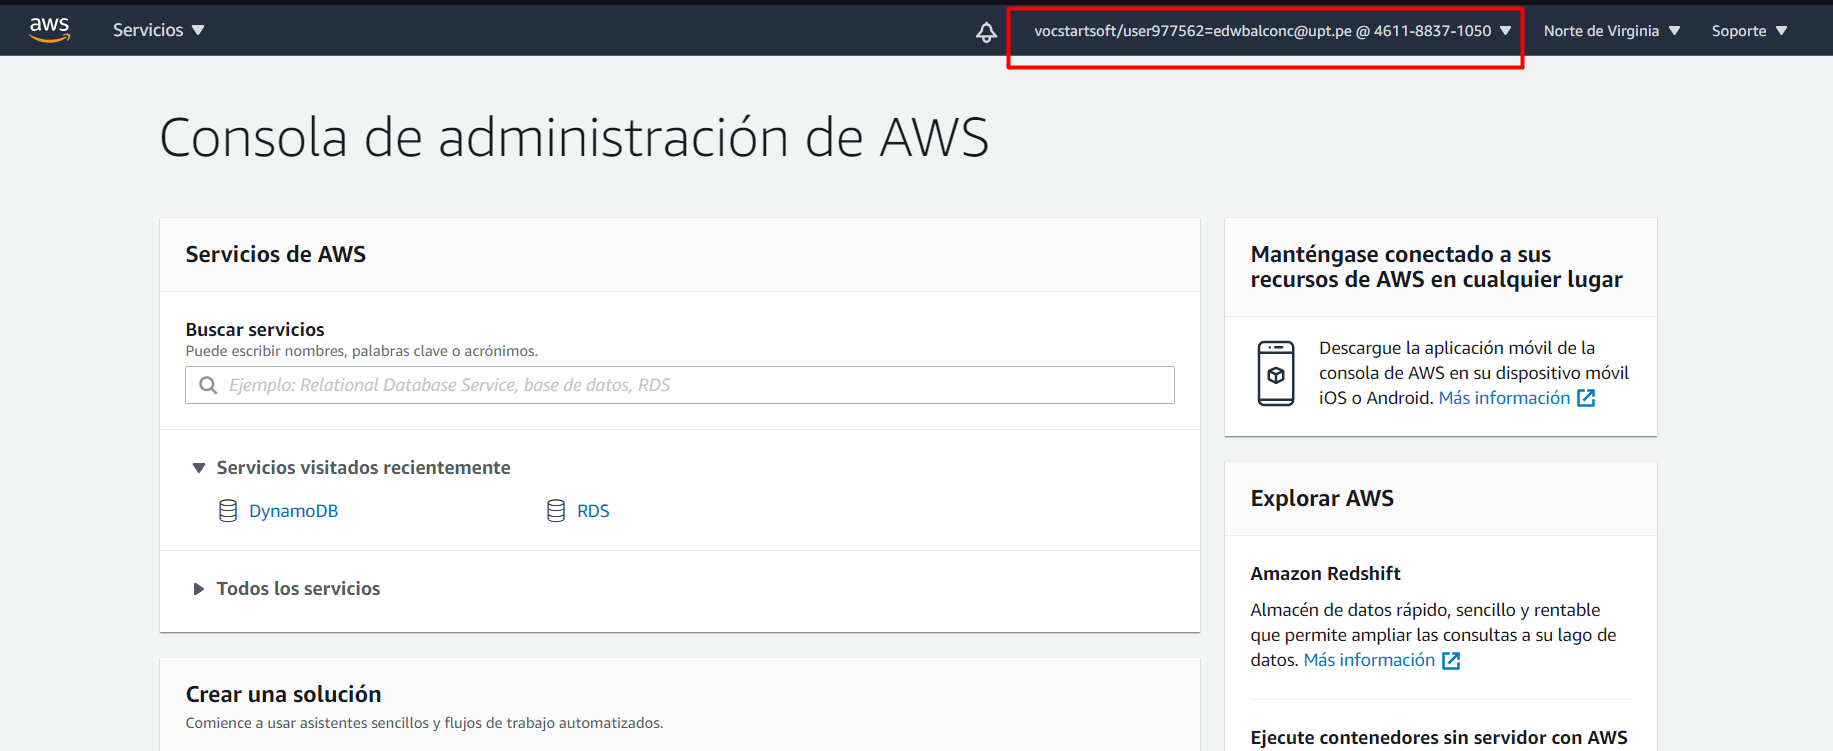
\includegraphics[width=15cm]{./images/1} 
	\end{center}
		\newpage
\textbf{1.2. 
Utilice el selector de región en la barra de navegación para elegir la región de AWS donde desea implementar el clúster de MongoDB en AWS. Para obtener más información, consulte Regiones, zonas de disponibilidad y zonas locales.}

    \begin{center}
		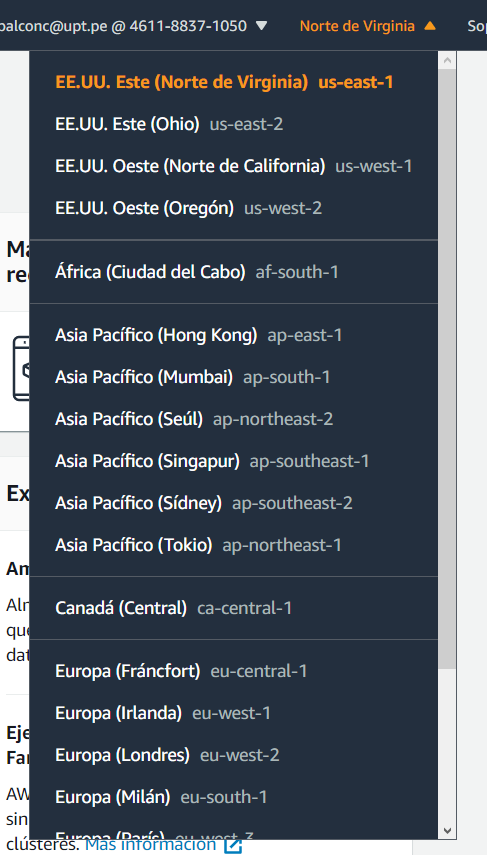
\includegraphics[width=7cm]{./images/2} 
	\end{center}
\newpage
\textbf{1.3. Cree un par de claves en su región preferida. Para hacer esto, en el panel de navegación de la consola de Amazon EC2, elija Key Pairs, Create Key Pair, escriba un nombre y luego elija Create.

}

    \begin{center}
		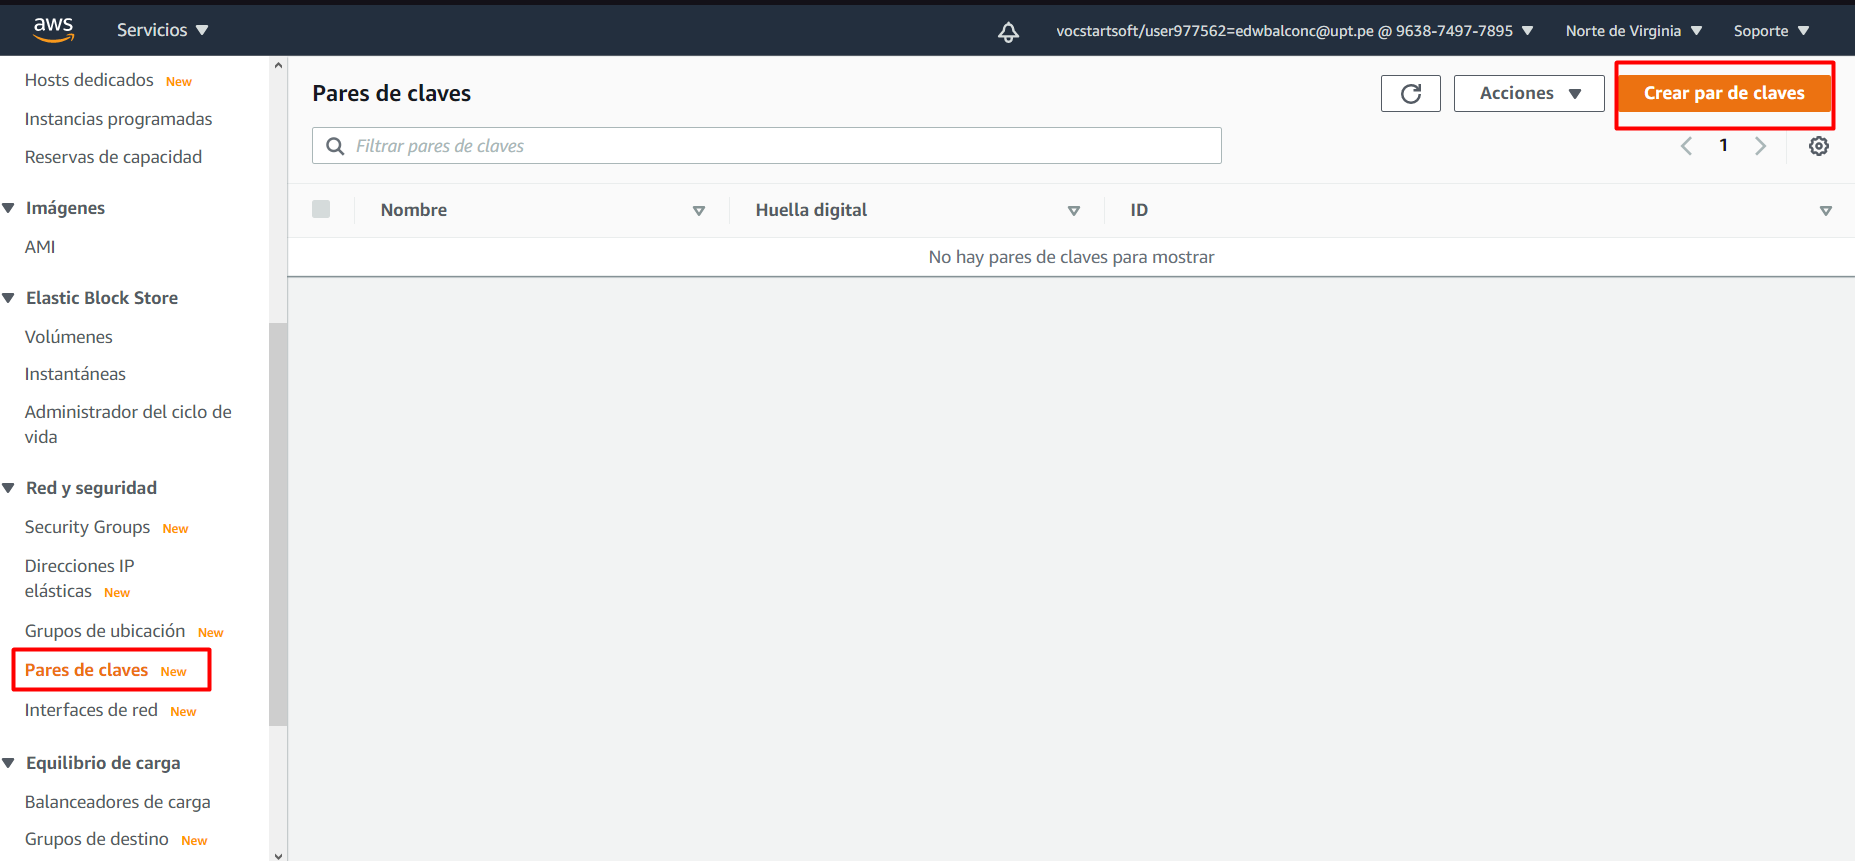
\includegraphics[width=15cm]{./images/3} 
	\end{center}
	 \begin{center}
		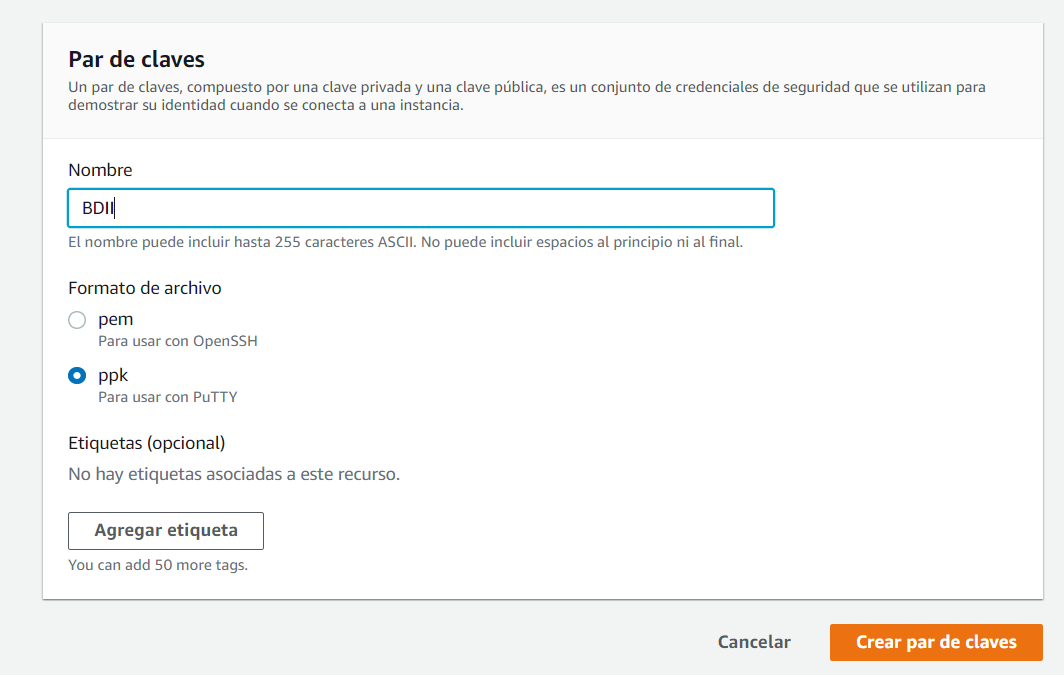
\includegraphics[width=15cm]{./images/4} 
	\end{center}

\begin{center}
		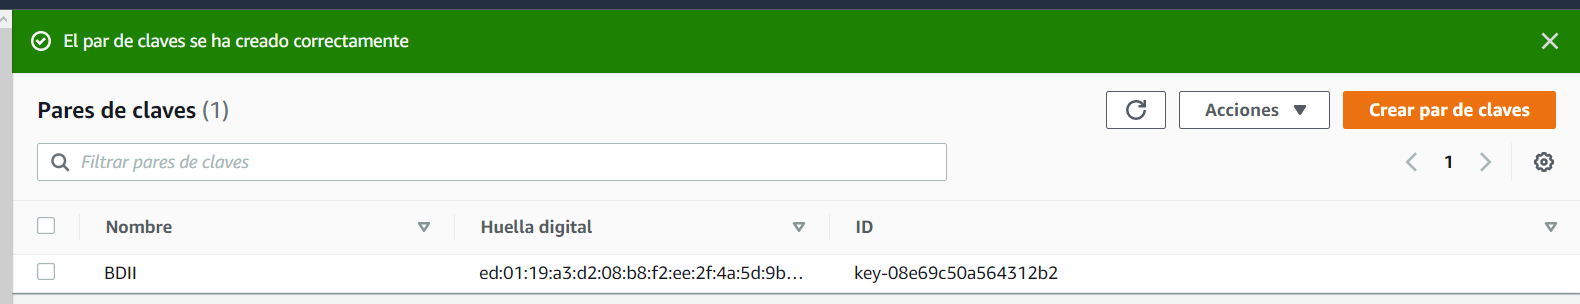
\includegraphics[width=15cm]{./images/5} 
	\end{center}
	
\newpage
\section{Inicio rápido }
\textbf{2.1. 
Elija una de las siguientes opciones para lanzar la plantilla de AWS CloudFormation en su cuenta de AWS. Para obtener ayuda para elegir una opción, consulte Opciones de implementación anteriormente en esta guía.}
    \begin{center}
		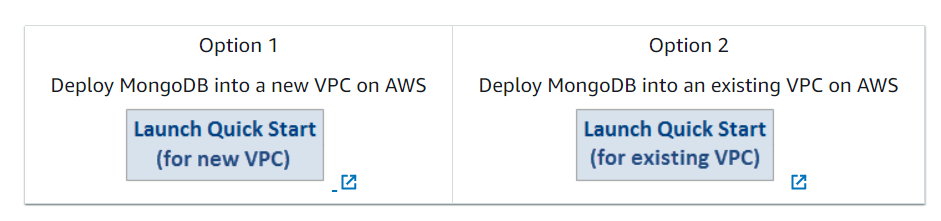
\includegraphics[width=15cm]{./images/6} 
	\end{center}
\textbf{2.2.
Verifique la región que se muestra en la esquina superior derecha de la barra de navegación y cámbiela si es necesario. La plantilla se lanza en la región de EE.UU.Este (Norte de Virginia) de forma predeterminada.}

    \begin{center}
		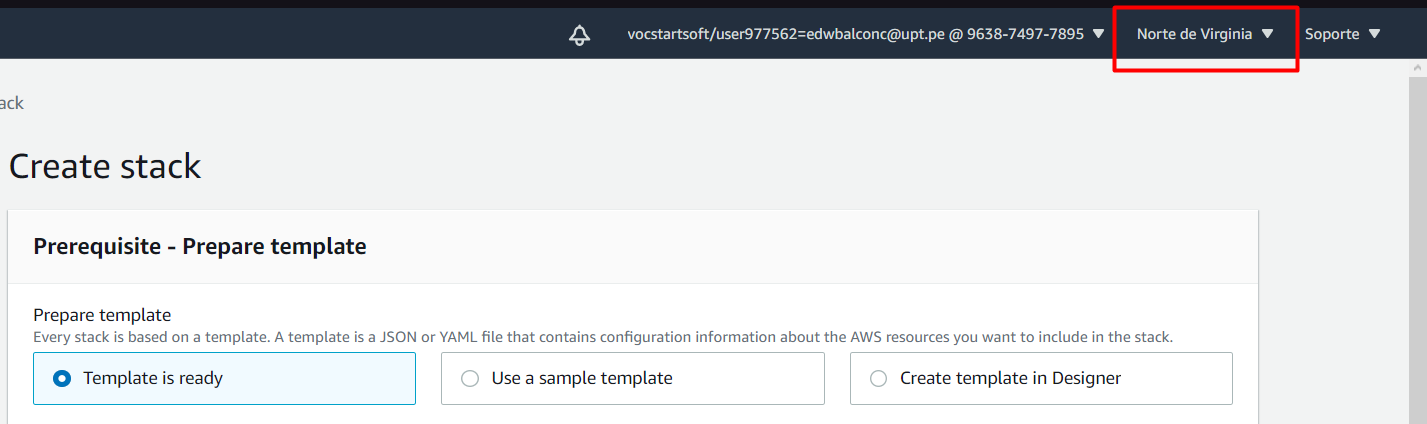
\includegraphics[width=15cm]{./images/7} 
	\end{center}
	
\newpage
\textbf{2.3.En la página Seleccionar plantilla, mantenga la configuración predeterminada para la URL de la plantilla y luego elija Siguiente.
}

    \begin{center}
		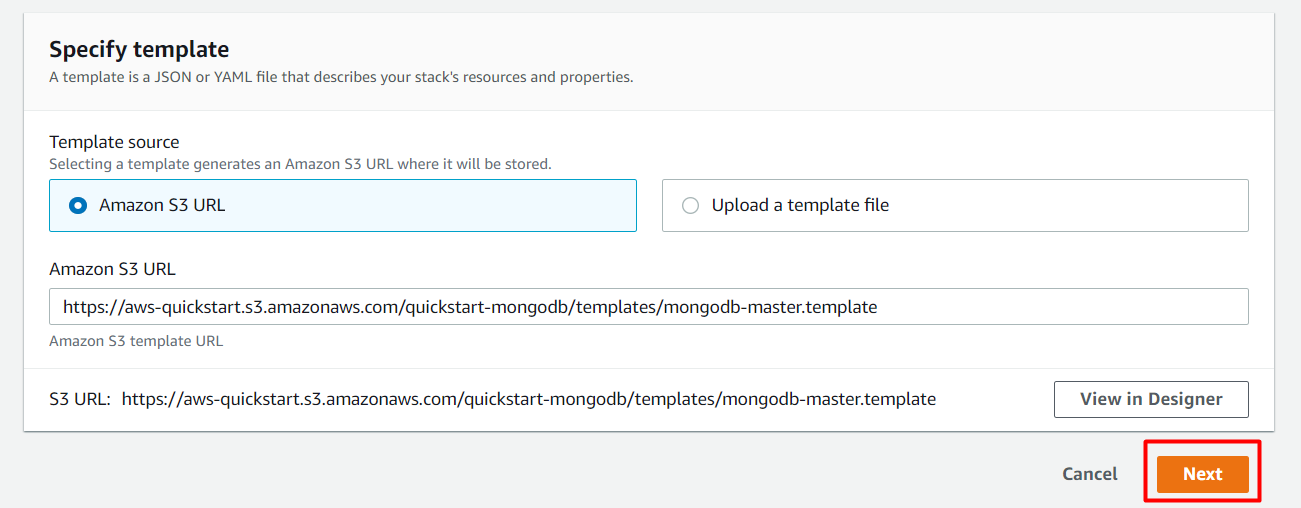
\includegraphics[width=15cm]{./images/8} 
	\end{center}
\newpage
\textbf{2.4. En la página Especificar detalles, cambie el nombre de la pila si es necesario. Revise los parámetros de la plantilla. Proporcione valores para los parámetros que requieren su entrada. Para todos los demás parámetros, revise la configuración predeterminada y personalícela según sea necesario. Cuando termine de revisar y personalizar los parámetros, elija Siguiente.
}

    \begin{center}
		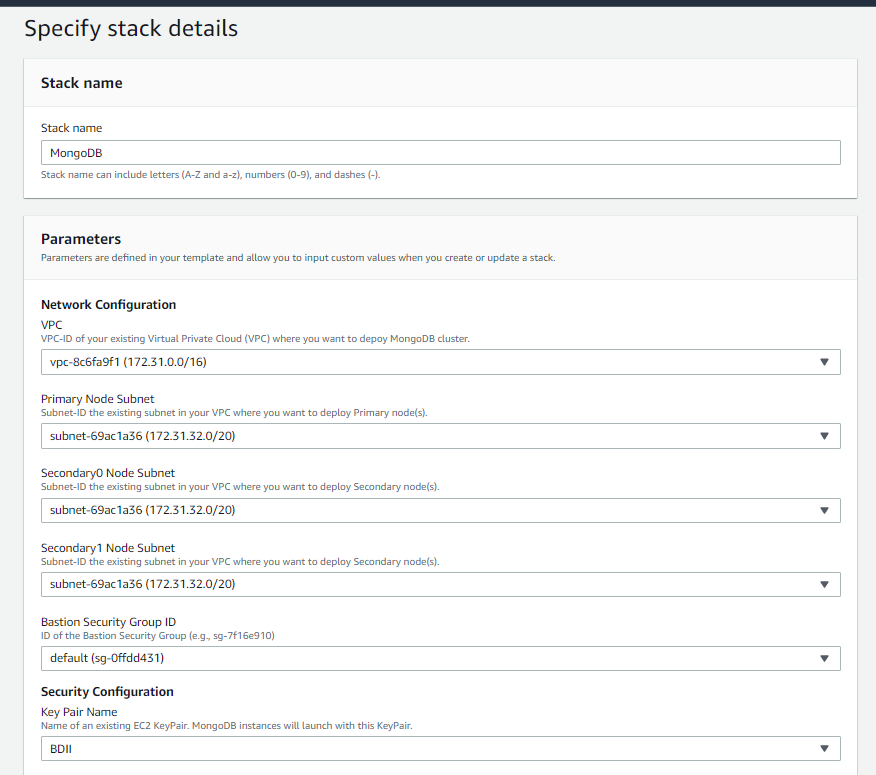
\includegraphics[width=15cm]{./images/t1} 
	\end{center}
	\begin{center}
		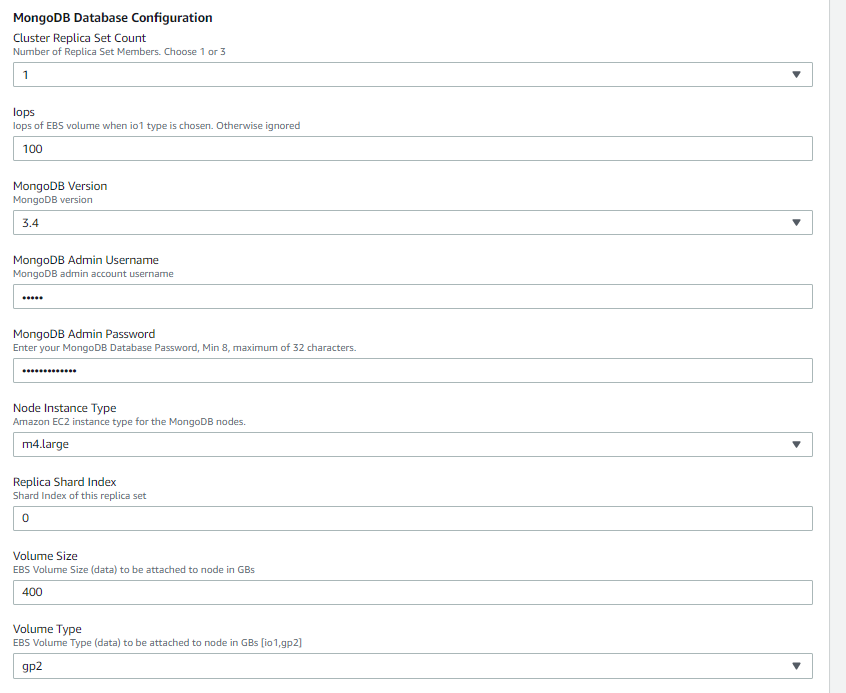
\includegraphics[width=15cm]{./images/t2} 
	\end{center}


\textbf{2.5. 
En la página Opciones, puede especificar etiquetas (pares clave-valor) para recursos en su pila y establecer opciones avanzadas. Cuando haya terminado, elija Siguiente. }

    \begin{center}
		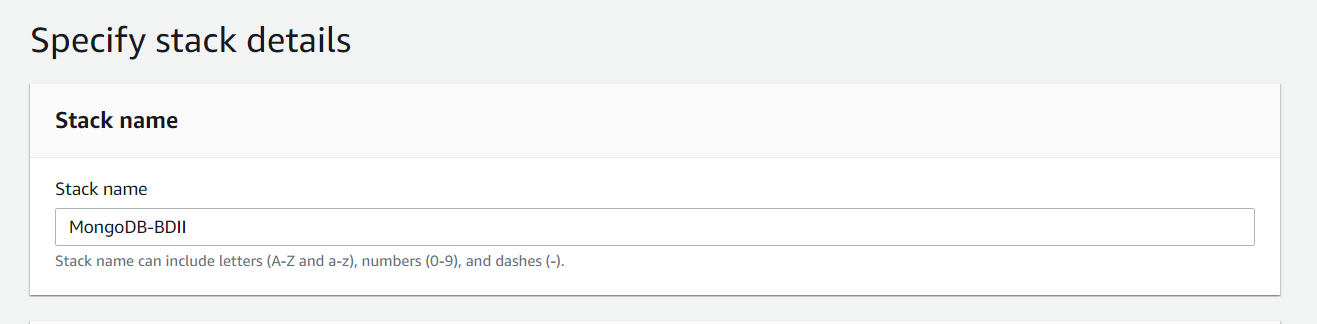
\includegraphics[width=15cm]{./images/9} 
	\end{center}
	\begin{center}
		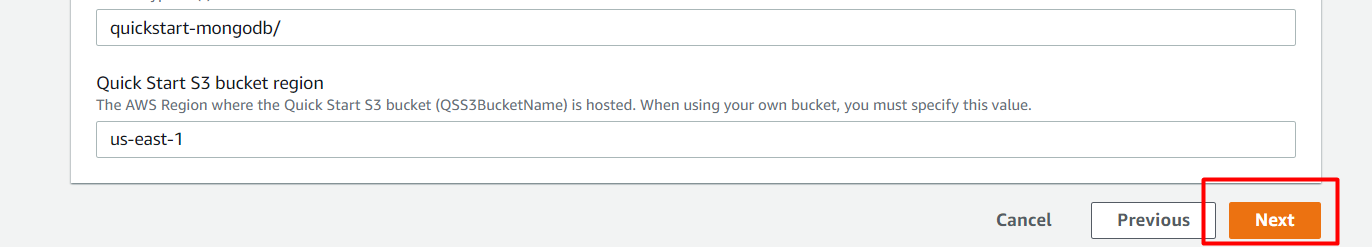
\includegraphics[width=15cm]{./images/10} 
	\end{center}
	\begin{center}
		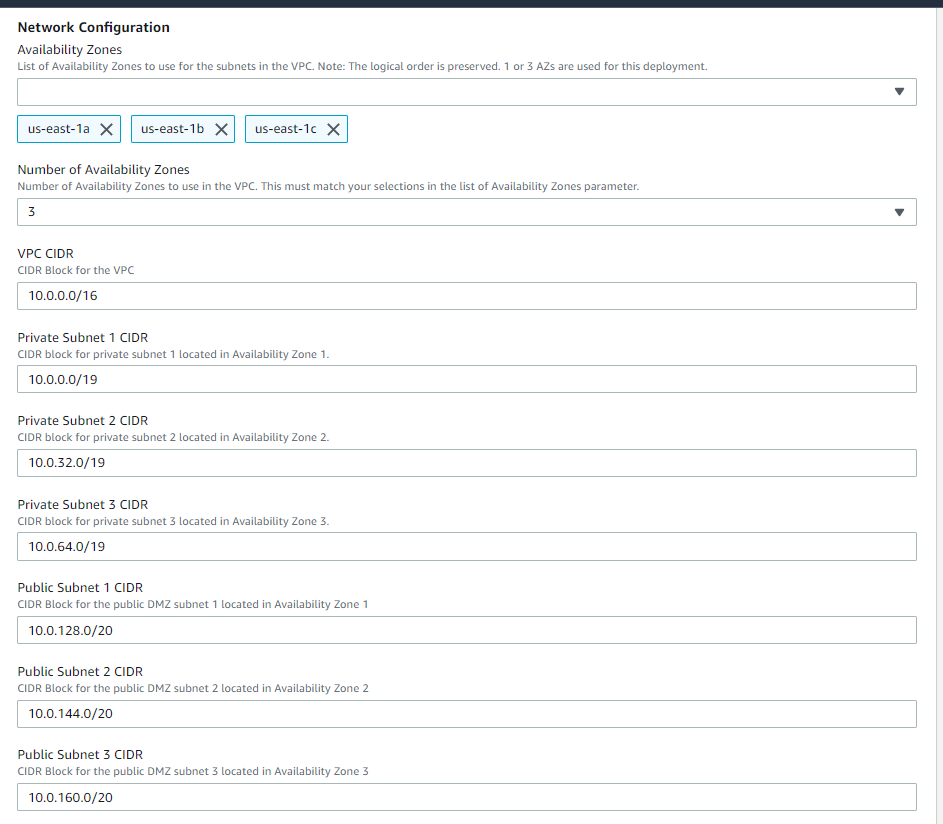
\includegraphics[width=15cm]{./images/11} 
	\end{center}
	\begin{center}
		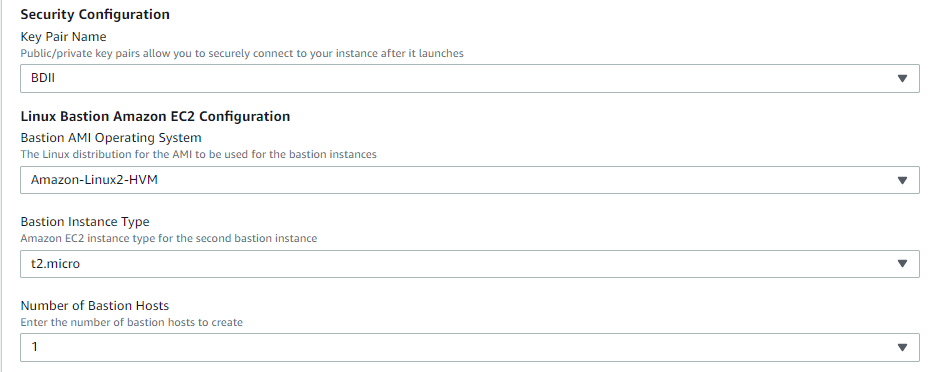
\includegraphics[width=15cm]{./images/12} 
	\end{center}
	
	\newpage
\textbf{2.6.En la página Revisar, revise y confirme la configuración de la plantilla. En Capacidades, seleccione la casilla de verificación para reconocer que la plantilla creará recursos de IAM. }

\begin{center}
		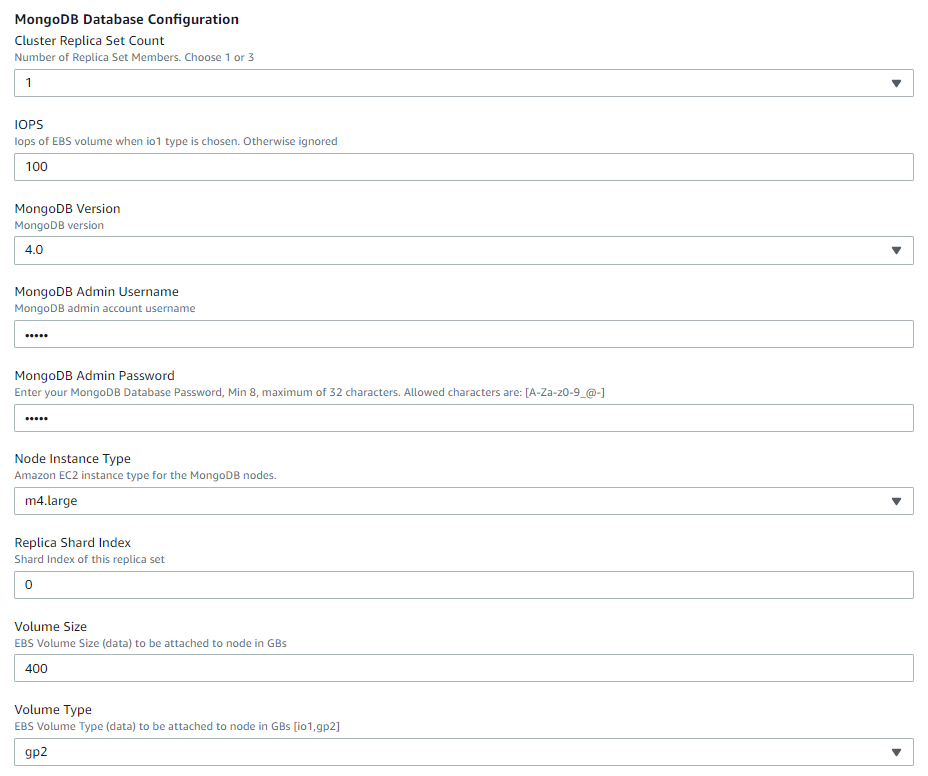
\includegraphics[width=15cm]{./images/13} 
	\end{center}
	\begin{center}
		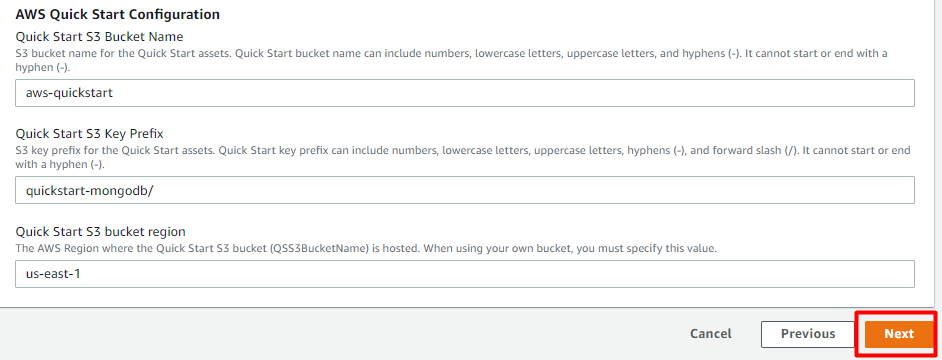
\includegraphics[width=15cm]{./images/14} 
	\end{center}
	
    \begin{center}
		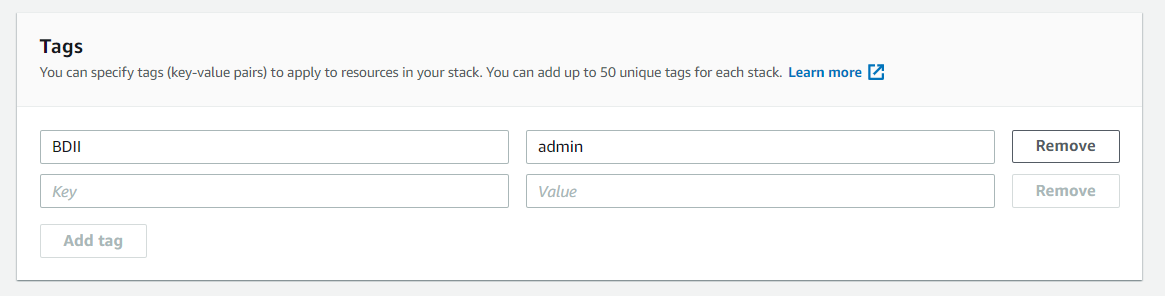
\includegraphics[width=15cm]{./images/15} 
	\end{center}
\textbf{2.7. Elija Crear para implementar la pila.
}

    \begin{center}
		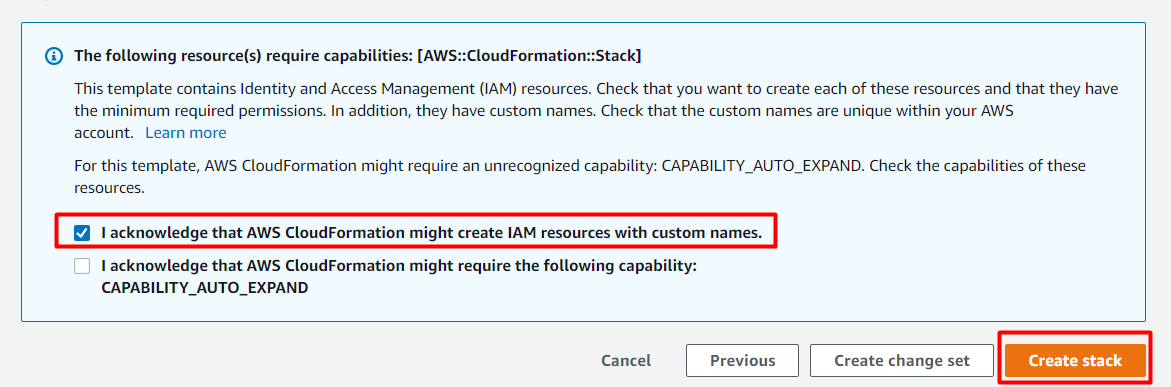
\includegraphics[width=15cm]{./images/16} 
	\end{center}

\newpage
\textbf{2.8. Supervise el estado de la pila. Cuando el estado es CREATE COMPLETE, como se muestra en la Figura 6, el clúster de MongoDB está listo.
}

    \begin{center}
		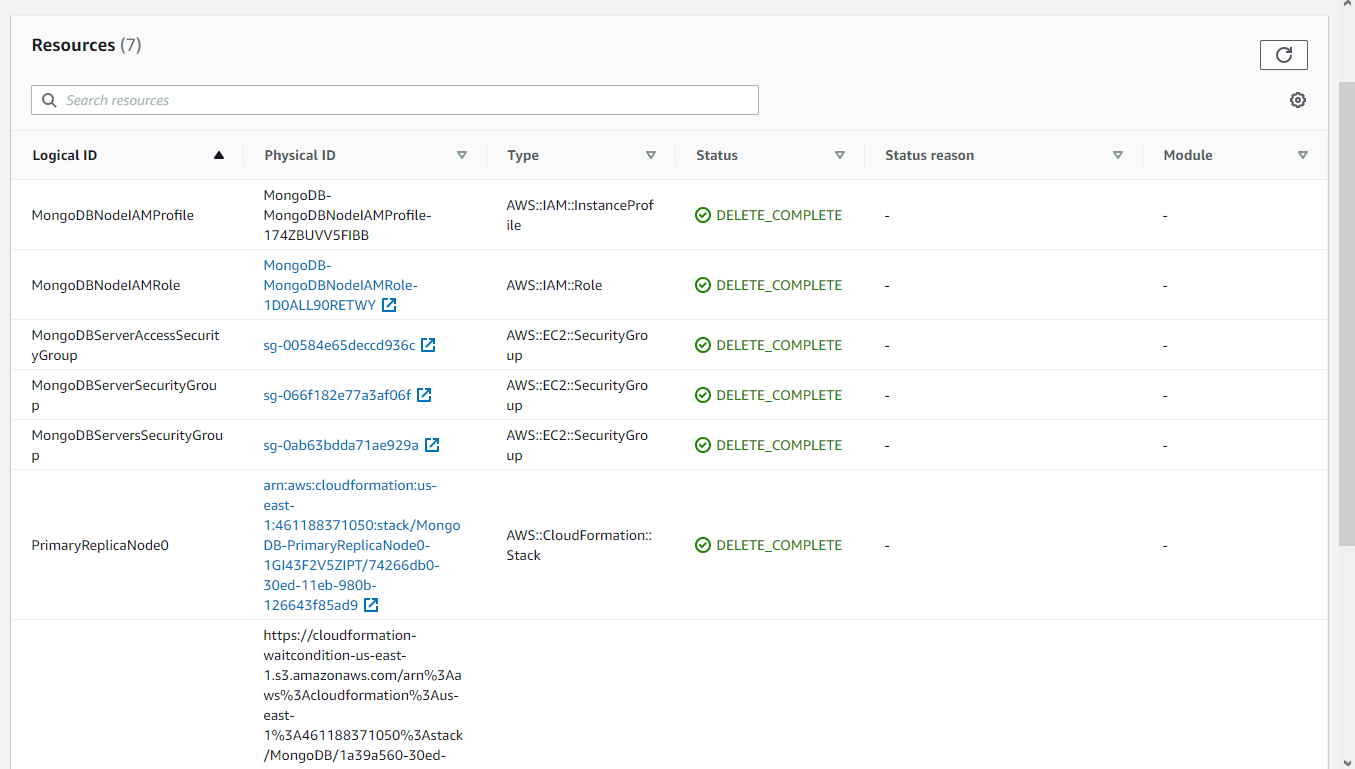
\includegraphics[width=15cm]{./images/17} 
	\end{center}


\end{document}